% !TeX root = ../../main.tex
% !TEX spellcheck = en_GB

\section{Design}
\label{ch:Design}
\begin{figure}
	\centering
	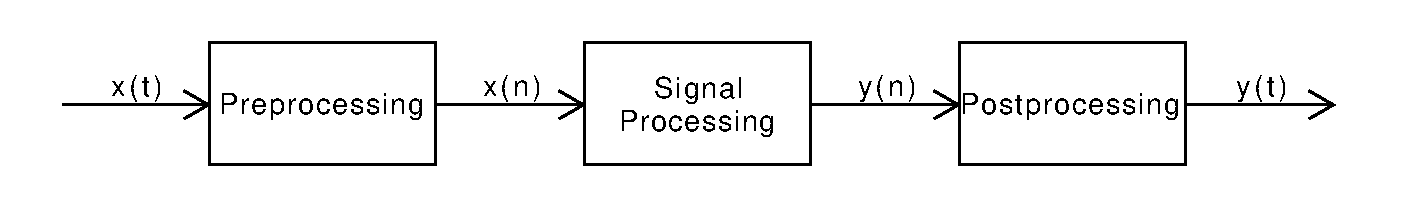
\includegraphics[width=1\linewidth]{gfx/Design/OverallDesign.pdf}
	\caption{Overall design of \systemName.}
	\label{fig:overalldesign}
\end{figure}

To fulfil the requirements specified, the system is split into three parts: Preprocessing, Signal processing and Post-processing, as seen in \cref{fig:overalldesign}.

\paragraph{Preprocessing} handles the analog to digital conversion and preprocessing allowing compliance with Non-functional requirement R1 and R2 for the Signal processing block.
This means Preprocessing takes the input, processes it and outputs a discrete signal which can be processed and modulated.

\paragraph{Signal processing} finds the frequency/tone based on the frequency found it shall be moved to the nearest corresponding C-major tone, shown in \cref{tab:cmajor}.

\paragraph{Post-processing} handles the digital to analog conversion.

\subsection{Detailed description of the design parts}
\subsubsection{Preprocessing}
On \cref{fig:DetailedPrePro} it can be seen that the analog signal will be sampled with a sampling frequency of \SI{48}{\kilo\hertz}.
The discrete signal wil be passed on to the FFT, which will make an FFT of the signal.
The FFT signal, xfft, will be passed on to the Hilbert max frequency determination block.
The Hilbert transform will find the dominating frequency in the signal.
Hilbert transform will only work when the input signal is a pure sine wave, if there are more sine waves mixed together it will find the average frequency and therefore a misinterpretation of the signal will be made.
Hilbert transformation requires many heavy calculations and deviations which will result in a product quantization error.
The found max frequency, maxFreq will be passed on to the signal processing block.

\begin{figure}
	\centering
	\includegraphics[width=1\linewidth]{gfx/Design/DesignPrePro_IF.pdf}
	\caption{Detailed description of Preprocessing in \systemName.}
	\label{fig:DetailedPrePro}
\end{figure}

\subsubsection{Signal processing}
\cref{fig:DetailedSigPro} shows the detailed idea of the signal processing part.

\begin{figure}
	\centering
	\includegraphics[width=1\linewidth]{gfx/Design/DesignSigPro_IF.pdf}
	\caption{Detailed description of Signal processing in \systemName.}
	\label{fig:DetailedSigPro}
\end{figure}

The maxFreq will be passed on to a Sinus generator, where it will be determined which frequency to go to on \cref{tab:cmajor}.
A sine wave with the found frequency will then be made with as few points as possible.
The generated sine wave, y(n), will be interpolated so the signal gets a lot of values in the sine wave, this method has been chosen with the thought that generating a sine wave with many points is more costly then interpolating.
The new full sine wave will be passed on to a circular buffer.
The idea behind the circular buffer is to avoid calculating the same sine wave again and again.
If the maxFreq appears to be the same multiple times, the sine wave in the circular buffer can be reused thus we do not have to generate or interpolate a new sine.
The output from the circular buffer will be the new complete discrete signal.

\subsubsection{Post processing}
The last phase of the system will take the final discrete signal and through a DAC make it to an analog signal as shown on \cref{fig:DetailedPostPro}.
\begin{figure}
	\centering
	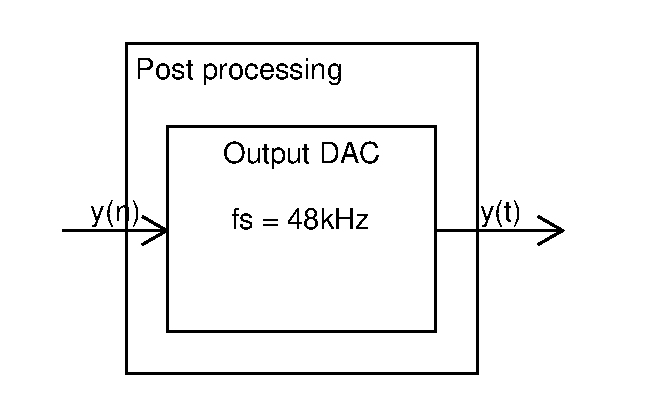
\includegraphics[width=1\linewidth]{gfx/Design/DesignPostPro_IF.pdf}
	\caption{Detailed description of Post processing in \systemName.}
	\label{fig:DetailedPostPro}
\end{figure}

\subsection{Quantization} 
There will be a quantization error on the IIR low pass filter, but since the filter is not steep and have rather long time to get to the stop band, the low pass filter does not suffer significantly from the quantization, as can be seen in \cref{fig:quant_error_filter} where the max difference was found to be $\SI{<0.5}{\percent} $.
Thus the quantization error for this specific filter is negligible, but the implementation this filter should be a FIR low pass filter since it is what works with the build in functions.

\begin{figure}
	\centering
	\includegraphics[width=1\linewidth]{gfx/QuantizationFilter.png}
	\caption{Matlab filter coefficients results in the red curve, 1.15 format in the yellow.}
	\label{fig:quant_error_filter}
\end{figure}
\fxnote{Matlab rød, 1.15 gul?}

In the filter there will occur coefficient and product quantization. Coefficient quantization will occur when the filter coefficients are fitted to the 1.15 format.
The product quantization will occur when the filter coefficients are multiplied with the data.
This will result in quantization since it still has to fit 1.15 format.
On \cref{fig:quant_error} the places where quantization occurs can be seen.

\begin{figure}
	\centering
	\includegraphics[width=1\linewidth]{gfx/Design/flow_quant_error.pdf}
	\caption{Quantization errors \systemName.}
	\label{fig:quant_error}
\end{figure}

\FloatBarrier